\documentclass{article}
\usepackage[utf8]{inputenc}
\usepackage[hidelinks]{hyperref}
\usepackage{graphicx, booktabs, setspace, dirtree, varwidth, listings, perpage, hyperref}

\MakePerPage{footnote}

\renewcommand{\contentsname}{Indice}
\renewcommand{\figurename}{Figura}

\newsavebox{\asciiart}
\newcommand{\showasciiart}{
	\raisebox{1\height}{
		\resizebox{80.5ex}{!}{\usebox{\asciiart}}
	}
}

\title{Relazione del progetto \texttt{Wordle}}
\author{Riccardo Mori}
\date{Marzo 2023}
\makeatletter

\begin{document}
	
	\begin{titlepage}
		\centering
		
\includegraphics[height=12pc]{img/marchio_unipi.pdf} \\
		\null
		\textsc{\huge Dipartimento di Informatica}
		\vfill
		{\huge{\@title}}
		\vfill
		\emph{Autore:} \@author \\
		\emph{Matricola:} 505163 \\
		\@date
	\end{titlepage}
	
	\setstretch{1.15}
	\tableofcontents
	\setstretch{1.0}
	\pagebreak
	
	\section{Descrizione del progetto}
Il progetto consiste nell'implementazione (in Java 8) di una versione semplificata del famoso gioco \textbf{Wordle}. In particolare questa variante del gioco supporta numero di tentativi e lunghezza delle parole variabili\footnote{I valori sono impostati staticamente (\emph{hardcoded})}. \newline
Il progetto si compone di due parti indipendenti fra loro: il \textbf{server} e il \textbf{client}.

La struttura e' la seguente:
\bigskip

\dirtree{%
	.1 /.
	.2 client/ \quad \begin{minipage}[t]{7cm}
		Implementazione del client
	\end{minipage}.
	.3 backend/ \hfill \begin{minipage}[t]{7cm}
		Offre un'implementazione di base delle funzionalita'
		supportate dal client
			\end{minipage}.
	.4 exceptions/.
	.3 frontend/ \hfill \begin{minipage}[t]{7cm}
		Implementazione frontend
	\end{minipage}.
	.4 CLI/ \quad \begin{minipage}[t]{7cm}
		Command Line Interface
	\end{minipage}.
	.4 GUI/ \quad \begin{minipage}[t]{7cm}
		Graphical User Interface (Opzionale)
	\end{minipage}.
	.2 protocol/ \hfill \begin{minipage}[t]{7cm}
		Costanti e strutture dati condivise relative al
		protocollo di comunicazione client-server over TCP
	\end{minipage}.
	.2 rmi/ \quad \begin{minipage}[t]{7cm}
		Interfacce e strutture dati condivise relative
		a RMI
	\end{minipage}.
	.3 exceptions/.
	.2 server/ \hfill \begin{minipage}[t]{7cm}
		Implementazione del server
	\end{minipage}.
	.3 logging/.
	.2 utils/ \quad \begin{minipage}[t]{7cm}
		Utilities
	\end{minipage}.
}
	\section{Protocollo di comunicazione}
Il protocollo di comunicazione client-server e' stato implementato avendo come obiettivi:
\begin{itemize}
	\item La dimensione dei messaggi inviati
	\item La facilita' del parsing dei messaggi
	\item L'indipendenza del protocollo da qualsiasi implementazione, linguaggio di programmazione, sistema operativo o architettura utilizzata
\end{itemize}

\begin{lrbox}{\asciiart}
	\begin{varwidth}{\maxdimen}
		\noindent\lstinputlisting[basicstyle=\ttfamily]{proto_fmt1.txt}
	\end{varwidth}
\end{lrbox}%

E' stato dunque scelto un protocollo custom binario in cui i messaggi vengono codificati in \textbf{UTF-8} e incapsulati all'interno di un pacchetto (come si puo' vedere in Figura \ref{fig:proto_fmt1}) nel seguente formato:
\begin{enumerate}
	\item Dimensione in byte del messaggio codificato in 4 bytes $BIG\_ENDIAN$
	\item Il messaggio vero e proprio (codificato in \emph{UTF-8})
\end{enumerate}

\begin{center}
	\begin{figure}[t!]
		\makebox[\textwidth]{\showasciiart{}}
		\caption{Rappresentazione dell'incapsulamento di un messaggio.}
		\label{fig:proto_fmt1}
	\end{figure}
\end{center}

Per una descrizione approfondita del formato dei messaggi consultare l'appendice \ref{appendix:format}
	\section{Server}

\subsection{Architettura}

\begin{center}
	\begin{figure}[t]
		\makebox[\textwidth]{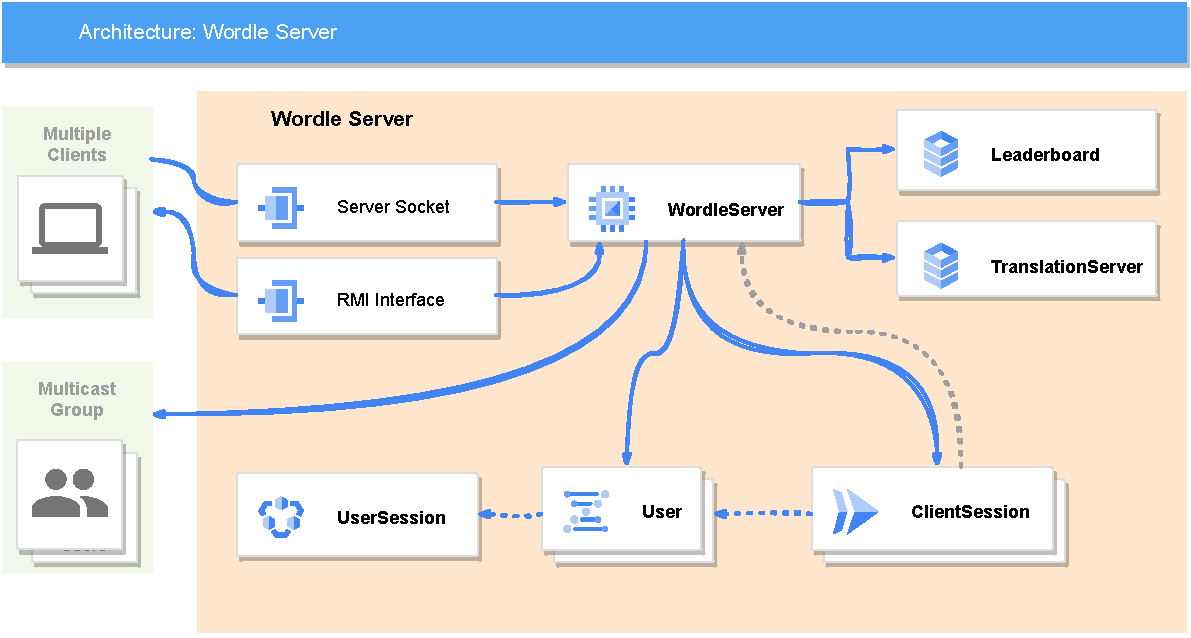
\includegraphics[width=0.7\paperwidth]{img/server_arch.pdf}}
		\caption{Rappresentazione dell'architettura del server. La linea tratteggiata blu indica che il riferimento e' opzionale (potrebbe non essere presente). Si noti che esiste una dipendenza circolare tra \textbf{WordleServer} e \textbf{ClientSession}: sarebbe stato possibile evitarla rendendo \textbf{ClientSession} una classe \texttt{private static} di \textbf{WordleServer}, ma si perderebbe in chiarezza.}
		\label{fig:server_arch}
	\end{figure}
\end{center}

La struttura del server (raffigurata in figura \ref{fig:server_arch}) e' la seguente:
\bigskip

\dirtree{%
	.1 server/.
	.2 ServerMain \quad \begin{minipage}[t]{7cm}
		Entry point principale
	\end{minipage}.
    .2 WordleServer \quad \begin{minipage}[t]{7cm}
    	Core del server, istanza singleton
    \end{minipage}.
	.2 ClientSession \quad \begin{minipage}[t]{7cm}
		Gestisce la sessione di un client
	\end{minipage}.
	.2 Leaderboard \quad \begin{minipage}[t]{7cm}
		Struttura dati che contiene la classifica degli utenti
	\end{minipage}.
	.2 TranslationServer \quad \begin{minipage}[t]{7cm}
		Offre la traduzione in italiano delle secret word
	\end{minipage}.
	.2 User \quad \begin{minipage}[t]{7cm}
		Rappresenta un utente
	\end{minipage}.
	.2 UserSession \quad \begin{minipage}[t]{7cm}
		La sessione di un utente
	\end{minipage}.
	.2 logging/.
}
\bigskip

Il nucleo principale del server e' contenuto nella classe \textbf{WordleServer} che e' anche un oggetto singleton poiche' deve essere istanziato la prima volta da \textbf{ServerMain} e da quel momento in poi non deve essere mai piu' istanziato nuovamente, ne' terminato.

\newpage

\textbf{WordleServer} si occupa di:
\begin{itemize}
	\item Gestione della comunicazione con i client (tramite TCP, UDP e java RMI)
	\item Mantenimento delle informazioni persistenti relative agli utenti
	\item Registrazione e autenticazione degli utenti
	\item Generazione e validazione delle parole segrete
	\item Condivisione delle partite nel gruppo di multicast\footnote{Vedi l'appendice \ref{appendix:udp_format} per una descrizione dettagliata del formato dei messaggi}
	\item Traduzione della \emph{secret word}
	\item Notificare i client (\emph{subscribers}) quando avviene un cambiamento nelle prime posizioni in classifica
\end{itemize}

Tuttavia \textbf{WordleServer} non e' direttamente responsabile della logica della interazione con i client che invece e' affidata a \textbf{ClientSession}, il quale e' stato implementato come un semplice automa a stati finiti (raffigurato in Figura \ref{fig:clientsession_asf}), cosa che permette di verificarne facilmente la correttezza e quindi di garantire che il client si trovera' sempre in uno stato \emph{"safe"}.

\begin{center}
	\begin{figure}[t!]
		\makebox[\textwidth]{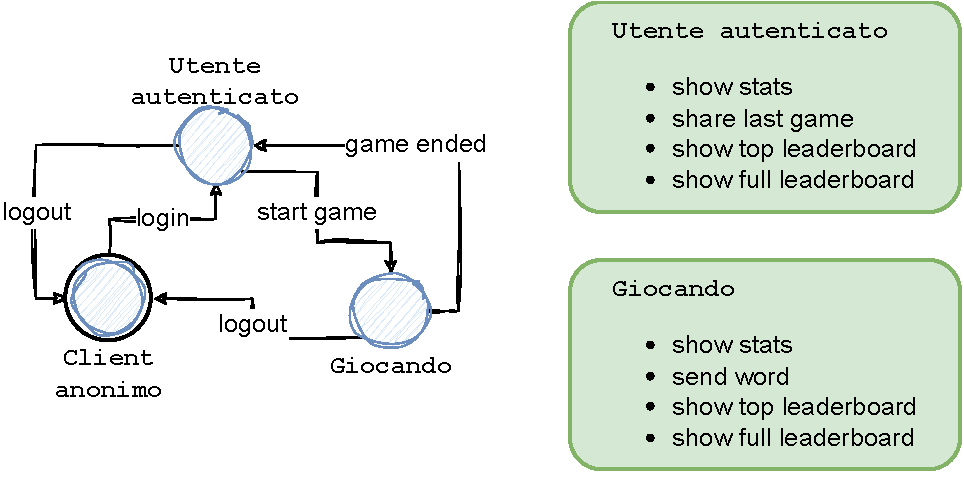
\includegraphics[width=0.6\paperwidth]{img/client_asf_v3.pdf}}
		\caption{A sinistra: descrizione dell'automa a stati finiti che gestisce l'interazione di un client con il server (lo stato iniziale e' quello cerchiato). A destra: elenco dei comandi validi in ogni stato (questi comandi non cambiano lo stato corrente dell'automa).}
		\label{fig:clientsession_asf}
	\end{figure}
\end{center}

\subsection{TCP Socket}

Si e' scelto di gestire le connessioni TCP con dei socket I/O non bloccanti (\emph{Java NIO}) piuttosto che avere un pool di thread in cui ogni thread e' responsabile di un solo client.

Questa soluzione ci permette una migliore scalabilita' con il numero di client, infatti un elevato numero di client che effettuano, tuttavia, poche operazioni causerebbe un enorme overhead se usassimo un thread ciascuno. In questo modo siamo limitati da un solo thread che gestisce le connessioni con dei dati pronti a essere letti o scritti.

In realta' la limitazione del thread singolo potrebbe essere rimossa qualora si sentisse il bisogno\footnote{Questa soluzione non e' stata adottata poiche' un tale livello di efficienza esula dagli obiettivi di questo progetto e l'implementazione risulta particolarmente insidiosa, tuttavia il resto del codice e' gia' stato predisposto per supportare una gestione parallela dei client} di migliorare ulteriormente l'efficienza sfruttando il parallelismo hardware (piu' core/CPU). In tal caso basterebbe delegare l'esecuzione di ciascun \textbf{ClientSession} a un pool di thread introducendo delle misure di sincronizzazione per evitare di elaborare due volte lo stesso messaggio.

\subsection{Leaderboard}

La classifica degli utenti e' gestita dalla classe \textbf{Leaderboard}. Internamente la classifica viene codificata con due strutture dati:
\begin{itemize}
	\item Un \textbf{BST} (\emph{Binary Search Tree}) in cui i nodi (che rappresentano gli utenti) sono ordinati per il \textbf{punteggio} dell'utente e sono etichettati con il relativo \textbf{username} (che ricordiamo essere unico)
	\item Una \textbf{hashmap} in cui la chiave e' lo \textbf{username} (se e solo se e' presente in classifica) e il valore associato e' un riferimento al nodo nel \textbf{BST} che identifica proprio quello username.
\end{itemize}
In questo modo sapere la posizione in classifica di un utente richiede $O(n)$ tempo mentre l'aggiunta, la rimozione e la modifica di una coppia (utente, punteggio) richiede $O(\log{n})$ tempo.

Vale la pena notare che usare un \textbf{Order Statistic Tree} al posto del \textbf{BST} comporterebbe un miglioramento della complessita' dell'operazione di \emph{rank}, ovvero sapere la posizione in classifica di un utente, che diventerebbe quindi $O(\log{n})$. Siccome l'implementazione di un \textbf{OST} non e' presente nella standard library di Java, questa soluzione non e' stata utilizzata.

Praticamente l'implementazione non rispecchia totalmente la struttura definita sopra ma comporta alcune piccole modifiche che non cambiano la complessita' del problema:
\begin{itemize}
	\item Il \textbf{BST} e' stato implementato mediante una \textbf{TreeMap} in cui la chiave e' la coppia (ordinabile lessicograficamente) \emph{(punteggio, username)} mentre il valore non e' utilizzato.
	\item La \textbf{hashmap} e' stata implementata tramite una \textbf{HashMap} la cui chiave e' uno \emph{username} e il valore e' la coppia \emph{(punteggio, username)}.
\end{itemize}
Per mantenere sincronizzate entrambe le strutture dati e' necessario che tutti i metodi della classe \textbf{Leaderboard} siano mutualmente esclusivi, per fare cio' e' sufficiente dichiararli \textbf{synchronized}.

\subsection{Traduzione della secret word}

La traduzione della \emph{secret word} (gestita dalla classe \textbf{TranslationServer}) in italiano e' una procedura lenta che richiede di eseguire una richiesta HTTP e dal momento che si e' deciso di non utilizzare un thread pool per la gestione concorrente dei client, l'intero server si blocca in attesa della risposta dal web server.

Per mitigare questo problema internamente viene usata una cache \textbf{LRU} (\emph{Least Recently Used}) che contiene la traduzione delle secret word. L'implementazione della cache \textbf{LRU} e' basata sulla \textbf{LinkedHashMap} offerta dalla standard library.

\subsection{Gestione della concorrenza}

Come precedentemente anticipato non ci sono molti thread che lavorano in parallelo. Tuttavia, alcune componenti sono eseguite in un thread separato, in particolare la lista dei thread e':
\begin{itemize}
	\item Il main thread
	\item Flush scheduler: viene eseguito a intervalli regolari ed esegue la sincronizzazione con il file di salvataggio del server
	\item Thread per la generazione di una nuova secret word. Anche questo viene eseguito a intervalli regolari
	\item Shutdown hook: thread speciale che viene eseguito nel momento in cui il server inizia la fase di terminazione. Esegue un sync sul file di salvataggio.
	\item Share game: il thread si occupa di condividere una partita nel gruppo di multicast. Essendo questa di per se' una attivita' asincrona puo' essere eseguita tranquillamente da un thread separato
	\item Notifica ai subscribers. Anche questa attivita' puo' essere eseguita parallelamente dal momento che non viene generata direttamente da un client
	\item RMI threads: I metodi remoti disponibili possono generare molteplici thread. Il threadpool in questo caso e' gestito dalla \emph{JVM}
\end{itemize}

E' quindi necessario fare in modo che non si presentino situazioni di deadlock ne' altri problemi.

La maggior parte di questi thread opera su strutture dati dedicate o su tipi di dato primitivi (l'assegnamento in tal caso e' atomico), quindi le misure per la prevenzione di problemi dovuti all'accesso concorrente alle risorse sono molto semplici o alle volte assenti.

L'unica struttura dati che merita particolare attenzione e' la \textbf{map} \{\emph{username} : \emph{User}\} che associa a ogni \emph{username} il relativo oggetto di tipo \emph{User} che rappresenta l'utente. Tale struttura e' particolarmente delicata per i seguenti motivi:
\begin{enumerate}
	\item In fase di registrazione bisogna garantire l'atomicita' dell'operazione di creazione di un utente se gia' non esiste
	\item L'autenticazione, che consiste nel controllare se un utente esiste e in tal caso controllare se la password e' valida, deve essere atomica
	\item Durante la sincronizzazione dello stato del server in un file di salvataggio e' necessario operare su uno snapshot della lista di utenti \textbf{evitando} di scrivere informazioni corrotte o parziali
	\item Ogni istanza di \textbf{ClientSession} puo' operare sul relativo oggetto \textbf{User} ma non opera direttamente sulla \textbf{map} \{\emph{username} : \emph{User}\}
\end{enumerate}

Per risolvere i punti 1-2 e mantenere comunque un alto livello di parallelismo si e' deciso di utilizzare una \textbf{ConcurrentHashMap}.
Ricordiamo infatti che valgono le seguenti proprieta':
\begin{itemize}
	\item Un utente, una volta registrato non puo' essere rimosso
	\item La password di un utente e' \emph{immutable}
\end{itemize}

Per quanto riguarda il punto 4 si e' deciso di imporre un'altra proprieta':
\begin{quote}
	 In ogni istante successivo alla inizializzazione del server \underline{solo un oggetto} di tipo \textbf{ClientSession} puo' operare su un determinato oggetto \textbf{User}
\end{quote}

Infine il punto 3 si risolve imponendo che la classe \textbf{User} sia serializzabile previa cattura del lock tramite \textbf{synchronized}. Questo significa che le operazioni di modifica su \textbf{User} sono tutte atomiche e lasciano l'oggetto in uno stato corretto.

\subsection{Configurazione}

Nel file di configurazione \texttt{ServerMain.properties} si possono configurare i seguenti valori:
\begin{itemize}
	\item \texttt{multicast\_address}: l'indirizzo del gruppo di multicast
	\item \texttt{multicast\_port}: la porta da utilizzare quando si mandano messaggi nel gruppo di multicast
	\item \texttt{server\_port}: la porta da usare per il server socket
	\item \texttt{rmi\_port}: la porta da usare per i servizi RMI
	\item \texttt{verbose}: la verbosita' dei log (da 0 a 5)
	\item \texttt{secret\_word\_rate}: l'intervallo in secondi tra la generazione di una secret word e la successiva
	\item \texttt{words\_db}: file contenente la lista di parole	
\end{itemize}
	\section{Client}

Il client e' diviso in due parti: \textbf{backend} e \textbf{frontend}. Il primo implementa tutte le varie funzioni che prevedono un'interazione con il server in modo da offrire una sorta di \emph{API} comune a qualsiasi frontend, il secondo invece e' l'interfaccia utente vera e propria.

Questa scelta permette di riutilizzare il codice e separare ulteriormente l'interfaccia dalle funzionalita'.

\subsection{Backend}

La struttura del backend e' la seguente:
\bigskip

\dirtree{%
	.1 client/backend/.
	.2 ClientBackend \quad \begin{minipage}[t]{7cm}
		Implementazione delle funzionalita' del client
	\end{minipage}.
	.2 NotificationListener \quad \begin{minipage}[t]{7cm}
		Riceve i messaggi da un gruppo di multicast
	\end{minipage}.
	.2 exceptions/ \quad \begin{minipage}[t]{7cm}
		Eccezioni custom
	\end{minipage}.
}
\bigskip

La classe principale e' ovviamente \textbf{ClientBackend} che implementa la quasi totalita' delle funzionalita' richieste dal client (login, inizio di una partita, tentativo di indovinare la parola segreta, ...). E' importante notare che le funzionalita' offerte \underline{non controllano} la consistenza dello stato del sistema ma sono una vera e propria \emph{API}. Sara' compito del frontend effettuare le chiamate giuste al momento giusto.

I metodi offerti da \textbf{ClientBackend} si occupano di creare il messaggio da inviare al server (tramite socket TCP) e in caso di successo terminano ritornando gli eventuali dati ricevuti dal server (corretamente parsati), altrimenti sollevano un'eccezione che estende \textbf{BackendException} indicativa del problema avvenuto. Nel caso in cui il messaggio di risposta dal server contenga dei dati aggiuntivi, nonostante l'operazione richiesta non sia andata a buon fine, tali dati, opportunamente parsati, verranno incapsulati all'interno dell'eccezione sollevata e potranno essere recuperati tramite il metodo \textbf{BackendException::getResult}. Se ne puo' vedere un esempio in \textbf{AlreadyPlayedException}.

Questo sistema permette una maggiore flessibilita' nella comunicazione tra \textbf{frontend} e \textbf{backend}, infatti l'utilizzatore del \textbf{backend} sapra' sempre qual e' il tipo di dato ritornato e quali le eccezioni generate. Alternativamente, ritornare sempre un tipo di dato che contemporaneamente codifichi (tipicamente tramite un intero) sia il successo che tutti i possibili errori e al tempo stesso anche tutti i possibili dati aggiuntivi comunicati dal server, avrebbe reso il codice meno leggibile, piu' prono a errori e meno auto-esplicativo.

Un'ultima considerazione va fatta per \textbf{NotificationListener} che lancia un thread nel quale resta in ascolto di eventuali messaggi su un gruppo multicast. Gli unici problemi causati dalla concorrenza in questo caso sono dovuti agli accessi alle risorse interne alla classe, quindi sono molto semplici da gestire.

\subsection{Frontend}

Il frontend e' offerto da due diverse implementazioni: una \textbf{CLI} (\emph{Command Line Interface}) e una \textbf{GUI} (\emph{Graphical User Interface}).

La \textbf{GUI}, essendo facoltativa, non verra' discussa nel dettaglio. Viene offerta \emph{as is} semplicemente per completezza.

La struttura del frontend e' la seguente:
\bigskip

\dirtree{%
	.1 client/frontend/.
	.2 CLI/.
	.3 ClientCLI.
	.2 ClientFrontend \quad \begin{minipage}[t]{7cm}
		Interfaccia che ogni frontend deve implementare
	\end{minipage}.
	.2 Command.
	.2 SessionState \quad \begin{minipage}[t]{7cm}
		Mantiene lo stato del client
	\end{minipage}.
	.2 GUI/.
}
\bigskip

Essendo che il client deve implementare l'interfaccia \textbf{clientRMI} in cui vengono specificati i metodi remoti che possono essere invocati dal server (che rappresenta una linea diretta di comunicazione col server), e' chiaro che il frontend dovra' implementare tali metodi, senza poter demandare al backend questa responsabilita'.

Fortunatamente c'e' solo un metodo (\textbf{updateLeaderboard}) invocabile da remoto ed e' di facile implementazione. Cio' non causa problemi di concorrenza.

Il resto del client e' composto da un singolo thread (il principale). Questo, unito al fatto che si appoggia al backend per l'implementazione delle funzionalita' richieste, rende la classe \textbf{ClientCLI} semplice e lineare.

\subsection{Configurazione}

Nel file di configurazione \texttt{ClientMain.properties} si possono configurare i seguenti valori:
\begin{itemize}
	\item \texttt{multicast\_address}: l'indirizzo del gruppo di multicast
	\item \texttt{multicast\_port}: la porta da utilizzare quando si mandano messaggi nel gruppo di multicast
	\item \texttt{server\_host}: l'host del server
	\item \texttt{server\_port}: la porta da usare per connettersi al server
	\item \texttt{rmi\_port}: la porta da usare per i servizi RMI
\end{itemize}
	\section{Manuale d'uso}

Per la compilazione e l'esecuzione e' richiesto \textbf{Java 8} o superiore.

Esistono diversi modi per compilare il progetto:
\begin{itemize}
	\item \hyperlink{makefile}{\textbf{Makefile}} (Linux, MacOS, Unix-like)
	\item \hyperlink{gradle}{\textbf{Gradle}} (All platforms)
	\item \hyperlink{manual}{\textbf{Manualmente}} (All platforms)
\end{itemize}

\hypertarget{makefile}{}
\subsection{Makefile}

\paragraph{Per compilare}
\begin{verbatim}
	$ make all
\end{verbatim}

\paragraph{Per creare i files \texttt{jar}}
\begin{verbatim}
	$ make jar
\end{verbatim}

Il risultato della compilazione sara' nella cartella \texttt{build/}

\bigskip
\bigskip
\hypertarget{gradle}{}
\subsection{Gradle}

\subsubsection{Unix}
Di seguito verra' descritta la procedura per sistemi Unix-like (Linux, MacOS, ...).

\paragraph{Per compilare}
\begin{verbatim}
	$ ./gradlew build
\end{verbatim}

Il risultato sara' nella cartella \texttt{app/build/}

\paragraph{Per creare i files \texttt{jar}}
\begin{verbatim}
	$ ./gradlew clientJar
	$ ./gradlew serverJar
\end{verbatim}

Il risultato sara' nella cartella \texttt{app/build/libs/}

\medskip
\subsubsection{Windows}
Di seguito verra' descritta la procedura per sistemi Windows.

\paragraph{Per compilare}
\begin{verbatim}
	gradlew.bat build
\end{verbatim}

Il risultato sara' nella cartella \texttt{app\textbackslash build\textbackslash}

\paragraph{Per creare i files \texttt{jar}}
\begin{verbatim}
	gradlew.bat clientJar
	gradlew.bat serverJar
\end{verbatim}

Il risultato sara' nella cartella \texttt{app\textbackslash build\textbackslash libs\textbackslash}

\bigskip
\bigskip
\hypertarget{manual}{}
\subsection{Metodo manuale}

\underline{\textbf{Non raccomandato}}

\subsubsection{Unix}
Di seguito verra' descritta la procedura per sistemi Unix-like (Linux, MacOS, ...).

\paragraph{Per compilare}
\begin{verbatim}
	$ javac -cp lib/gson-2.10.1.jar:./app/src/main/java: -d ./build \ 
	    app/src/main/java/edu/riccardomori/wordle/server/ServerMain.java
	$ javac -cp lib/gson-2.10.1.jar:./app/src/main/java: -d ./build \
	    app/src/main/java/edu/riccardomori/wordle/client/ClientMain.java
\end{verbatim}

Il risultato sara' nella cartella \texttt{app/build/}

\medskip
\subsubsection{Windows}
Di seguito verra' descritta la procedura per sistemi Windows.

\paragraph{Per compilare}
\begin{verbatim}
	javac.exe -cp lib\gson-2.10.1.jar;.\app\src\main\java; -d .\build \ 
	app\src\main\java\edu\riccardomori\wordle\server\ServerMain.java
	javac.exe -cp lib\gson-2.10.1.jar:.\app\src\main\java: -d .\build \
	app\src\main\java\edu\riccardomori\wordle\client\ClientMain.java
\end{verbatim}

Il risultato sara' nella cartella \texttt{app\textbackslash build\textbackslash}

\bigskip
\subsection{Esecuzione}

Per eseguire l'applicazione e' \underline{consigliato} usare i file \texttt{jar} precedentemente compilati nel seguente modo:
\begin{verbatim}
	$ java -jar client.jar
	$ java -jar server.jar
\end{verbatim}

Altrimenti e' possibile lanciare l'applicazione manualmente nel seguente modo:

\paragraph{Unix:}
\begin{verbatim}
	$ java -cp lib/gson-2.10.1.jar:./build/ \
	     edu.riccardomori.wordle.client.ClientMain
	$ java -cp lib/gson-2.10.1.jar:./build/ \
	     edu.riccardomori.wordle.server.ServerMain
\end{verbatim}


\paragraph{Windows:}
\begin{verbatim}
	java.exe -cp lib\gson-2.10.1.jar;.\build edu.riccardomori.wordle.client.ClientMain
	java.exe -cp lib\gson-2.10.1.jar;.\build edu.riccardomori.wordle.server.ServerMain
\end{verbatim}

	\section{Note}

Il codice in questione si puo' trovare all'indirizzo \url{https://github.com/patacca/wordle-Unipi}

La versione qui descritta e' quella identificata dal commit \href{https://github.com/patacca/wordle-Unipi/commit/b9383070a42909956722c58ba582b070cc9e75a3}{b938307}
	
	\newpage
	
	\appendix
	\section{Formato dei messaggi}
\label{appendix:format}

\paragraph{NOTA:} Tutti i messaggi sono codificati in \textbf{UTF-8} e i valori sono codificati in \emph{BIG\_ENDIAN}
\paragraph{Legenda:}
\begin{itemize}
	\item Il simbolo \textbf{B} indica l'unita' \texttt{byte}
	\item Qualora il nome del campo sia racchiuso tra \textbf{[} e \textbf{]} significa che la sua lunghezza e' variabile
	\item I campi marcati dal simbolo \textbf{*} sono opzionali
	\item Tutti e soli i valori di \textbf{MESSAGE\_STATUS} sono descritti nella classe \texttt{protocol/MessageStatus.java}
\end{itemize}

\paragraph{Importante:} Tutti i messaggi di risposta del server sono nel seguente formato:

\begin{lrbox}{\asciiart}
	\begin{varwidth}{\maxdimen}
		\noindent\lstinputlisting[basicstyle=\ttfamily]{format/base_server.txt}
	\end{varwidth}
\end{lrbox}%

\begin{center}
	\begin{figure}[h]
		\makebox[\textwidth]{\showasciiart{80ex}}
		\centering \textbf{MESSAGE\_STATUS} rappresenta l'esito dell'operazione e \textbf{SERVER\_DATA} e' un campo di lunghezza variabile presente solo in alcuni casi.
	\end{figure}
\end{center}

Di seguito verranno descritti i messaggi del client e \underline{solo} i messaggi \textbf{SERVER\_DATA} nel caso siano presenti.

\newpage

\subsection{Login}

\paragraph{Messaggio inviato dal client}

\begin{lrbox}{\asciiart}
	\begin{varwidth}{\maxdimen}
		\noindent\lstinputlisting[basicstyle=\ttfamily]{format/login_client.txt}
	\end{varwidth}
\end{lrbox}%

\begin{center}
	\begin{figure}[h]
		\makebox[\textwidth]{\showasciiart{80.5ex}}
		\centering \textbf{U\_SIZE} e \textbf{P\_SIZE} rappresentano rispettivamente la lunghezza in bytes del campo \textbf{USERNAME} e \textbf{PASSWORD}
	\end{figure}
\end{center}

\paragraph{Messaggio inviato dal server}

---

\subsection{Start Game}

\paragraph{Messaggio inviato dal client}

\begin{lrbox}{\asciiart}
	\begin{varwidth}{\maxdimen}
		\noindent\lstinputlisting[basicstyle=\ttfamily]{format/startgame_client.txt}
	\end{varwidth}
\end{lrbox}%

\begin{center}
	\begin{figure}[h]
		\makebox[\textwidth]{\showasciiart{40ex}}
	\end{figure}
\end{center}

\paragraph{Messaggio inviato dal server}

\begin{lrbox}{\asciiart}
	\begin{varwidth}{\maxdimen}
		\noindent\lstinputlisting[basicstyle=\ttfamily]{format/startgame_server.txt}
	\end{varwidth}
\end{lrbox}%

\begin{center}
	\begin{figure}[h]
		\makebox[\textwidth]{\showasciiart{50ex}}
		\centering \textbf{SECRET\_LEN} indica il numero di caratteri di cui e' composta la \emph{secret word}. \textbf{N\_TRIES} e' il numero di tentativi concessi.
	\end{figure}
\end{center}

\newpage

\subsection{Logout}

\paragraph{Messaggio inviato dal client}

\begin{lrbox}{\asciiart}
	\begin{varwidth}{\maxdimen}
		\noindent\lstinputlisting[basicstyle=\ttfamily]{format/logout_client.txt}
	\end{varwidth}
\end{lrbox}%

\begin{center}
	\begin{figure}[h]
		\makebox[\textwidth]{\showasciiart{40ex}}
	\end{figure}
\end{center}

\paragraph{Messaggio inviato dal server}

---

\subsection{Send Word}

\paragraph{Messaggio inviato dal client}

\begin{lrbox}{\asciiart}
	\begin{varwidth}{\maxdimen}
		\noindent\lstinputlisting[basicstyle=\ttfamily]{format/sendword_client.txt}
	\end{varwidth}
\end{lrbox}%

\begin{center}
	\begin{figure}[h]
		\makebox[\textwidth]{\showasciiart{50ex}}
	\end{figure}
\end{center}

\paragraph{Messaggio inviato dal server}

\subparagraph{Se l'utente ha gia' terminato la partita per la secret word corrente}

\begin{lrbox}{\asciiart}
	\begin{varwidth}{\maxdimen}
		\noindent\lstinputlisting[basicstyle=\ttfamily]{format/sendword_server1.txt}
	\end{varwidth}
\end{lrbox}%

\begin{center}
	\begin{figure}[h]
		\makebox[\textwidth]{\showasciiart{45ex}}
		\centering \textbf{NEXT\_GAME\_TIME} e' l'orario espresso in \emph{unix time} in millisecondi in cui verra' generata la nuova \emph{secret word}.
	\end{figure}
\end{center}


\subparagraph{Se la parola inviata non e' valida}

\begin{lrbox}{\asciiart}
	\begin{varwidth}{\maxdimen}
		\noindent\lstinputlisting[basicstyle=\ttfamily]{format/sendword_server2.txt}
	\end{varwidth}
\end{lrbox}%

\begin{center}
	\begin{figure}[h]
		\makebox[\textwidth]{\showasciiart{45ex}}
		\centering Numero di tentativi rimasti.
	\end{figure}
\end{center}

\newpage

\subparagraph{Altrimenti}

\begin{lrbox}{\asciiart}
	\begin{varwidth}{\maxdimen}
		\noindent\lstinputlisting[basicstyle=\ttfamily]{format/sendword_server3.txt}
	\end{varwidth}
\end{lrbox}%

\begin{center}
	\begin{figure}[h]
		\makebox[\textwidth]{\showasciiart{85ex}}
		\centering \textbf{N\_TRIES} e' il numero di tentativi rimasti. \textbf{C\_SIZE} e \textbf{P\_SIZE} sono la dimensione di \textbf{CORRECT\_HINT} e \textbf{PARTIAL\_HINT}.
	\end{figure}
\end{center}

Il formato di \textbf{CORRECT\_HINT} e \textbf{PARTIAL\_HINT} e' lo stesso ed e' una serie di bytes che indicano la posizione (0-based) del carattere rispettivamente corretto, o presente ma in posizione sbagliata


\subsection{Get Stats}

\paragraph{Messaggio inviato dal client}

\begin{lrbox}{\asciiart}
	\begin{varwidth}{\maxdimen}
		\noindent\lstinputlisting[basicstyle=\ttfamily]{format/stats_client.txt}
	\end{varwidth}
\end{lrbox}%

\begin{center}
	\begin{figure}[h]
		\makebox[\textwidth]{\showasciiart{40ex}}
	\end{figure}
\end{center}

\paragraph{Messaggio inviato dal server}

\begin{lrbox}{\asciiart}
	\begin{varwidth}{\maxdimen}
		\noindent\lstinputlisting[basicstyle=\ttfamily]{format/stats_server.txt}
	\end{varwidth}
\end{lrbox}%

\begin{center}
	\begin{figure}[h]
		\makebox[\textwidth]{\showasciiart{85ex}}
		\centering \textbf{GAMES} e' il numero totale di partite effettuate. \textbf{WON\_GAMES} e' il numero di partite vinte. \textbf{CURR\_STREAK} e' lo streak di vittorie attuale. \textbf{BEST\_STREAK} e' lo streak di vittorie piu' lungo. \textbf{SCORE} e' punteggio. \textbf{DIST\_SIZE} (codificato in 1 byte) e' la lunghezza della guess distribution.
	\end{figure}
\end{center}

La guess distribution e' codificata come una sequenza di interi (codificati in 4 bytes ognuno).

\subsection{Get Leaderboard}

\paragraph{Messaggio inviato dal client}

\begin{lrbox}{\asciiart}
	\begin{varwidth}{\maxdimen}
		\noindent\lstinputlisting[basicstyle=\ttfamily]{format/leaderboard_client.txt}
	\end{varwidth}
\end{lrbox}%

\begin{center}
	\begin{figure}[h]
		\makebox[\textwidth]{\showasciiart{40ex}}
	\end{figure}
\end{center}

\paragraph{Messaggio inviato dal server}

\begin{lrbox}{\asciiart}
	\begin{varwidth}{\maxdimen}
		\noindent\lstinputlisting[basicstyle=\ttfamily]{format/leaderboard_server.txt}
	\end{varwidth}
\end{lrbox}%

\begin{center}
	\begin{figure}[h]
		\makebox[\textwidth]{\showasciiart{85ex}}
		\centering \textbf{NAME\_SIZE} e' la dimensione in bytes dello username. Le posizioni degli utenti sono gia' ordinate in base alla posizione in classifica.
	\end{figure}
\end{center}

\paragraph{Nota:} Esistono due operazioni distinte che il client puo' effettuare: richiedere la classifica intera o solo le prime posizioni (il numero esatto dipende dall'implementazione del server).
Il formato dei messaggi in entrambi i casi e' lo stesso, cambia solamente il codice del client (\textbf{5} per le prime posizioni, \textbf{6} per la classifica completa).

\subsection{Share game}

\paragraph{Messaggio inviato dal client}

\begin{lrbox}{\asciiart}
	\begin{varwidth}{\maxdimen}
		\noindent\lstinputlisting[basicstyle=\ttfamily]{format/share_client.txt}
	\end{varwidth}
\end{lrbox}%

\begin{center}
	\begin{figure}[h]
		\makebox[\textwidth]{\showasciiart{40ex}}
	\end{figure}
\end{center}

\paragraph{Messaggio inviato dal server}

---

\paragraph{Nota:} Esistono due operazioni distinte che il client puo' effettuare: richiedere la classifica intera o solo le prime posizioni (il numero esatto dipende dall'implementazione del server).
Il formato dei messaggi in entrambi i casi e' lo stesso, cambia solamente il codice del client (\textbf{5} per le prime posizioni, \textbf{6} per la classifica completa).


	
\end{document}
Symbols